\documentclass[oneside]{book}
\usepackage{epsfig,graphicx} % Required for inserting images
\usepackage{amsmath}
\usepackage{amsthm}
\usepackage{amssymb}
\usepackage{subcaption}
\usepackage[spanish,mexico]{babel}
\usepackage[bookmarksopen]{hyperref}
\usepackage[utf8]{inputenc}
\usepackage{array}
\usepackage{listings} %Soporte para código
\usepackage[left=2cm,right=2cm,top=1.8cm,bottom=2.3cm]{geometry}
\usepackage{titlesec}
\usepackage{fancyhdr} 
\usepackage{enumitem}
\usepackage{multicol}           % Permits header customization. See header section below.
\usepackage{multirow}           % Permits header customization. See header section below.
\usepackage{wrapfig}
\usepackage{bookmark}
\usepackage{sectsty}
% ---definición de los paquetes--
\fancypagestyle{plain}{
    \lhead{}
    \fancyhead[R]{\thepage}
    \fancyhead[L]{}
    \renewcommand{\headrulewidth}{0pt}
    \fancyfoot{}
}
\pagestyle{fancy}
\fancyhead[R]{	\thepage}
\fancyhead[L]{}
% Definir el tamaño del título del capítulo
\titleformat{\chapter}[display]
  {\normalfont\huge\bfseries} % Estilo del título
  {\chaptertitlename\ \thechapter}{1pt}{\Large} % Tamaño del título
  \titlespacing*{\chapter}{0pt}{-20pt}{20pt} % Ajustar el espaciado

\title{4ta lista de problemas}
\author{Ramírez Mendoza Joaquín Rodrigo\\
Treviño Puebla Héctor Jerome\\
Villalobos Juárez Gontrán Eliut
}
\date{\today}
% ---Inicio de la portada
\begin{document}
\begin{titlepage}

\begin{minipage}{3cm}
\begin{center}

\includegraphics[height = 0.14\textheight]{recursos/Logo_UNAM.png}\par
\end{center}
\end{minipage}\hfill
\begin{minipage}{10cm}

\end{minipage}\hfill
\begin{minipage}{3cm}
\begin{center}

\includegraphics[height = 0.14\textheight]{recursos/Logo_FC.png}\par
\end{center}
\end{minipage}
\centering
\vspace{1cm}

{\bfseries\LARGE Universidad Nacional Autónoma de México \par}

\vspace{1cm}
{\scshape\Large Facultad de Ciencias \par}
\vspace{1cm}
{\scshape\Large Matemáticas para las Ciencias Aplicadas 1 \par}
\vspace{1cm}
{\scshape\Large Licenciatura en Ciencias de la Computación \par}
\vspace{1cm}
{\scshape\Huge 4ta lista de problemas  \par}
\vspace{3cm}
{\itshape\Large Cuarto Parcial \par}
\vfill
{\Large Autores: \par}
{\Large Ramírez Mendoza Joaquín Rodrigo \par}
{\Large Villalobos Juárez Gontrán Eliut\par}
{\Large Treviño Puebla Héctor Jerome \par}
\vfill
{\Large Noviembre 2024 \par}
\end{titlepage}
% ---Fin de la portada de la portada
\maketitle

% Introducir aquí sus capítulos
\chapter*{Ejercicio 13 Cápitulo 5 ABD }

\textbf{13.-} Evalua la integral:
\[
\int \frac{x}{(x^{2}-1)\sqrt{x^{4}-2x^{2}}}dx
\]
Haciendo la sustitución de:
\[
u = x^{2}-1
\]
Así:
\begin{align*}
\frac{du}{dx} &= \frac{d}{dx}x^{2}-1 \\
\frac{du}{dx} &= 2x \\
du &= 2xdx  
\end{align*}
\newline
Para resolver esta integral, completaremos el T.C.P. (Trinomio Cuadrado Perfecto) que se encuentra adentro de la raíz de esta forma:
\begin{align*}
x^{4}-2x^{2} &= x^{4}-2x^{2} + 1 -1 \\
x^{4}-2x^{2} &= (x^{4}-2x^{2} + 1) -1 \\
x^{4}-2x^{2} &= (x^{2}-1)^{2}-1 \\
\end{align*}
Así nuestra integral resulta:
\[
\int \frac{x}{(x^{2}-1)\sqrt{(x^{2}-1)^{2}-1}}dx
\]
Ahora, podemos hacer uso de la Fórmula de 18 (Del formulario auorizado):
\[
\int \frac{du}{u\sqrt{u^{2}-a^{2}}} = \frac{1}{a}arcsec\frac{u}{a} + c
\]
Usando:
\begin{multicols}{2}
	\noindent
	\begin{align*}
		u^{2} &= (x^{2}-1)^{2} \\
        u  &= (x^{2}-1) \\
        du &= 2xdx \\
	\end{align*}
	\columnbreak
	\begin{align*}
		a^{2} &= 1 \\
        a &= 1 \\
	\end{align*}
\end{multicols}

De esta forma:
\begin{align*}
\int \frac{du}{u\sqrt{u^{2}-a^{2}}} &=   \int \frac{x}{(x^{2}-1)\sqrt{(x^{2}-1)^{2}-1}}dx \\
\int \frac{du}{u\sqrt{u^{2}-a^{2}}} &=   \frac{1}{2}\int \frac{2xdx}{(x^{2}-1)\sqrt{(x^{2}-1)^{2}-1}} \\
\end{align*}
Tenemos:
\begin{align*}
\frac{1}{a}arcsec\frac{u}{a} + c &=   \frac{1}{2}[\frac{1}{1}arcsec(\frac{x^{2}-1}{1}) + c] \\
\frac{1}{a}arcsec\frac{u}{a} + c &=   \frac{1}{2}arcsec (x^{2}-1) + c \\
\end{align*}
Resultado:
\[
\int \frac{x}{(x^{2}-1)\sqrt{x^{4}-2x^{2}}}dx = \frac{1}{2}arcsec (x^{2}-1) + c
\]

\chapter*{Ejercicio 53 Cápitulo 5 ABD }

\textbf{53.-} Usa la parte 2 del Teorema Fundamental del Calculo y (donde sea necesario) la Fórmula 18 de la Sección 5.10 para encontrar las derivadas: \\
\newline
Recordando:\\
2da Parte del Teorema Fundamental del Calculo en el ABD:
\[
\frac{d}{dx}\Bigl[\int_{a}^{b}f(t)dt \Bigr] = f(x)
\]
Fórmula 18 Sección 5.10 ABD:
\[
\frac{d}{dx}\Bigl[\int_{a}^{g(x)}f(t)dt \Bigr] = f(g(x))g'(x)
\]
Para el caso de este ejercicio (53) haremos uso de la fórmula 18:
\[
\frac{d}{dx}\Bigl[\int_{2}^{sen(x)}\frac{1}{1+t^{3}}dt \Bigr] 
\]
Con:
\begin{align*}
    g(x) &= sen (x) \\
    g'(x) &= cos (x) \\
\end{align*}
Así:
\[
f(g(x)) = \frac{1}{1+sen^{3}(x)}
\]
Por lo tanto:
\[
f(g(x))g'(x) = \frac{1}{1+sen^{3}(x)}(cos (x))
\]
El resultado es:
\[
\frac{d}{dx}\Bigl[\int_{2}^{sen(x)}\frac{1}{1+t^{3}}dt \Bigr] = \frac{cos(x)}{1+sen^{3}(x)}
\]
\chapter*{Ejercicio 68 Cápitulo 5 ABD }

\textbf{68.-} Una partícula se mueve a lo largo del eje-s. Use la informaciónd dada para encontrar la función posición del la partícula: \\
Información dada:
\begin{align*}
    a(t) &= 4cos(2t) \\
    v(0) &= -1 \\
    s(0) &= -3 \\
\end{align*}
Sabemos que al Integrar la Acelearción obtendremos la función de la velocidad de la partícula:
\begin{align*}
    v(t)&=\int a(t)dt \\
    v(t)&=\int 4cos(2t)dt \\
    v(t)&= 4\int cos(2t)dt \\
    \text{Con:} \\
    u   &= 2t \\
    du  &= 2dt \\
    v(t)&= 4\frac{1}{2}\int cos(2t)2dt \\
    v(t)&= \frac{4}{2}\int cos(2t)2dt \\
    v(t)&= 2sen(2t) + c\\
\end{align*}
Para hallar la constante de integración ($c$) y dar a $v(t)$, ocuparemos la evaluación que nos dieron de la velocidad en el tiempo $t=0$.
\begin{align*}
    v(0) = -1 &= 2sen(0) +c \\
    -1 &= 2(0) + c \\
    -1 &= c \\
\end{align*}
Así: 
\[
v(t) = 2sen(2t)-1
\]
Hacemos un proceso semejante para hallar la función posición $s(t)$.
Sabemos que al integrar la velocidad, obtendremos la posición.
\begin{align*}
    s(t)&=\int v(t)dt \\
    s(t)&=\int (2sen(2t) -1 )dt \\
    s(t)&= \int 2sen(2t)dt - \int dt  \\
    \text{Con:} \\
    u   &= 2t \\
    du  &= 2dt \\
    s(t)&= \frac{2}{2}\int sen(2t)dt - t + c \\
    s(t)&= -\frac{2}{2} cos(2t) - t + c \\
    s(t)&= - cos(2t) - t + c \\
\end{align*}
Para hallar la $c$, seguimos un proceso semejante al anterior:
\begin{align*}
    s(0) = -3 &= - cos(2(0)) - (0) + c \\
    -3 &= - cos(0)+ c  \\
    -3 &=  - 1 +c \\
    -3 +1 &= c \\
    -2 &= c \\
\end{align*}
Así conseguimos la función posición $s(t)$ que buscabamos:
\[
s(t) = -cos(2t)-t-2
\]

\chapter*{Ejercicio 85 Cápitulo 5 ABD }

\textbf{85.-} Evalua la integral hacienodo una sustitución apropieada:
\[
\int_{0}^{1} sen^{2}(\pi x)cos(\pi x) dx
\]
Para la sustitución tomaremos a $u$ como:
\[
u = sen(\pi x)
\]
Así:
\begin{align*}
    \frac{du}{dx} &= \frac{d}{dx}sen(\pi x) \\
    \frac{du}{dx} &= cos(\pi x) \pi \\
    du &= \pi cos(\pi x)  dx \\
\end{align*}

Así podemos usar la Fórmula 2 del formulario autorizado:
\[
\int u^{n}du = \frac{u^{n+1}}{n+1} +c \\
\]
Con esto:
\begin{align*}
    \int u^{n}du &= \int_{0}^{1} sen^{2}(\pi x)cos(\pi x) dx \\
    \int_{0}^{1} sen^{2}(\pi x)cos(\pi x) dx &= \frac{1}{\pi} \int_{0}^{1} sen^{2}(\pi x)\pi cos(\pi x) dx \\
    \int_{0}^{1} sen^{2}(\pi x)cos(\pi x) dx &= \frac{1}{\pi} \int_{0}^{1} sen^{2}(\pi x)\pi cos(\pi x) dx \\
    \int_{0}^{1} sen^{2}(\pi x)cos(\pi x) dx &= \frac{1}{\pi} \Bigl[\frac{sen^{3}(\pi x)}{3}\Bigr]_{0}^{1} \\
    \int_{0}^{1} sen^{2}(\pi x)cos(\pi x) dx &= \frac{1}{\pi} \Bigl[\frac{sen^{3}(\pi (1)}{3} - \frac{sen^{3}(\pi (0)}{3}\Bigr]\\
    \int_{0}^{1} sen^{2}(\pi x)cos(\pi x) dx &= \frac{1}{\pi} \Bigl[\frac{sen^{3}(\pi)}{3} - \frac{sen^{3}(0)}{3}\Bigr]\\
    \int_{0}^{1} sen^{2}(\pi x)cos(\pi x) dx &= \frac{1}{\pi} \Bigl[\frac{0}{3} - \frac{0}{3}\Bigr]\\
    \int_{0}^{1} sen^{2}(\pi x)cos(\pi x) dx &= \frac{1}{\pi} [0]\\
\end{align*}
Así el resultado de la integral es:
\[
\int_{0}^{1} sen^{2}(\pi x)cos(\pi x) dx = 0
\]

\chapter*{Ejercicios capitulo 5 ABD Grupo 3}

\section*{Ejercicio 42}
\textbf{Calcular el área bajo la curva \( y = \frac{1}{x} \) en el intervalo \([1, e^3]\).}

El área bajo la curva está dada por la integral definida:
\[
\int_{1}^{e^3} \frac{1}{x} \, dx
\]

\subsection*{Plantear la integral}
Tenemos:
\[
\int_{1}^{e^3} \frac{1}{x} \, dx
\]

\subsection*{Calcular la integral indefinida}
Sabemos que:
\[
\int \frac{1}{x} \, dx = \ln|x| + C
\]

\subsection*{Evaluar la integral definida}
Sustituimos los límites de integración:
\[
\int_{1}^{e^3} \frac{1}{x} \, dx = \left[ \ln x \right]_{1}^{e^3}
\]

\subsection*{Sustituir los límites}
Evaluamos en los límites:
\[
\left[ \ln x \right]_{1}^{e^3} = \ln(e^3) - \ln(1)
\]

\subsection*{Simplificar}
Sabemos que:
\[
\ln(e^3) = 3 \quad \text{y} \quad \ln(1) = 0
\]
Por lo tanto:
\[
\ln(e^3) - \ln(1) = 3 - 0 = 3
\]

\subsection*{Resultado final}
El área bajo la curva es:
\[
\boxed{3}
\]
\newpage

\section*{Ejercicio 64}
\textbf{Encontrar el valor promedio de \( f(x) = e^x + e^{-x} \) en el intervalo \([ \ln \frac{1}{2}, \ln 2 ]\).}

El valor promedio de una función está dado por:
\[
f_{\text{promedio}} = \frac{1}{b-a} \int_{a}^{b} f(x) \, dx
\]
En este caso, \( f(x) = e^x + e^{-x} \), \( a = \ln \frac{1}{2} \) y \( b = \ln 2 \).

\subsection*{Planteamiento}
Sustituimos en la fórmula:
\[
f_{\text{promedio}} = \frac{1}{\ln 2 - \ln \frac{1}{2}} \int_{\ln \frac{1}{2}}^{\ln 2} (e^x + e^{-x}) \, dx
\]

\subsection*{Simplificar los límites del denominador}
Sabemos que:
\[
\ln 2 - \ln \frac{1}{2} = \ln 2 - \ln 2^{-1} = \ln 2 + \ln 2 = 2 \ln 2
\]
Por lo tanto:
\[
f_{\text{promedio}} = \frac{1}{2 \ln 2} \int_{\ln \frac{1}{2}}^{\ln 2} (e^x + e^{-x}) \, dx
\]

\subsection*{Calcular la integral indefinida}
\[
\int (e^x + e^{-x}) \, dx = \int e^x \, dx + \int e^{-x} \, dx
\]
Resolviendo cada término:
\[
\int e^x \, dx = e^x, \quad \int e^{-x} \, dx = -e^{-x}
\]
Por lo tanto:
\[
\int (e^x + e^{-x}) \, dx = e^x - e^{-x} + C
\]

\subsection*{Evaluar la integral definida}
Sustituimos los límites:
\[
\int_{\ln \frac{1}{2}}^{\ln 2} (e^x + e^{-x}) \, dx = \left[ e^x - e^{-x} \right]_{\ln \frac{1}{2}}^{\ln 2}
\]

\subsection*{Sustituir los límites en la función}
Evaluamos:
\[
\left[ e^x - e^{-x} \right]_{\ln \frac{1}{2}}^{\ln 2} = \left( e^{\ln 2} - e^{-\ln 2} \right) - \left( e^{\ln \frac{1}{2}} - e^{-\ln \frac{1}{2}} \right)
\]
Simplificamos:
\[
e^{\ln 2} = 2, \quad e^{-\ln 2} = \frac{1}{2}, \quad e^{\ln \frac{1}{2}} = \frac{1}{2}, \quad e^{-\ln \frac{1}{2}} = 2
\]
Por lo tanto:
\[
\left( e^{\ln 2} - e^{-\ln 2} \right) - \left( e^{\ln \frac{1}{2}} - e^{-\ln \frac{1}{2}} \right) = \left( 2 - \frac{1}{2} \right) - \left( \frac{1}{2} - 2 \right)
\]
Simplificamos:
\[
\left( 2 - \frac{1}{2} \right) - \left( \frac{1}{2} - 2 \right) = \frac{3}{2} + \frac{3}{2} = 3
\]

\subsection*{Calcular el valor promedio}
Sustituimos en la fórmula del promedio:
\[
f_{\text{promedio}} = \frac{1}{2 \ln 2} \cdot 3 = \frac{3}{2 \ln 2}
\]

\subsection*{Resultado final}
El valor promedio es:
\[
\boxed{\frac{3}{2 \ln 2}}
\]
 \newpage 
 \section*{Ejercicio 76}

La función de velocidad dada es:
\[
v(t) = \frac{2}{5} \sqrt{5t + 1} + \frac{8}{5}.
\]

Queremos calcular el \textbf{desplazamiento} y la \textbf{distancia} recorrida por la partícula en el intervalo \( [0, 3] \).

\subsection*{Desplazamiento}

El desplazamiento se calcula como la integral de la velocidad:
\[
\text{Desplazamiento} = \int_{0}^{3} v(t) \, dt.
\]
Sustituimos \( v(t) \) en la integral:
\[
\int_{0}^{3} v(t) \, dt = \int_{0}^{3} \left( \frac{2}{5} \sqrt{5t + 1} + \frac{8}{5} \right) \, dt.
\]
Separando la integral:
\[
\int_{0}^{3} v(t) \, dt = \frac{2}{5} \int_{0}^{3} \sqrt{5t + 1} \, dt + \frac{8}{5} \int_{0}^{3} 1 \, dt.
\]

\subsubsection*{Primera integral: \( \int_{0}^{3} \sqrt{5t + 1} \, dt \)}

Sea \( u = 5t + 1 \), por lo tanto:
\[
du = 5 \, dt \quad \text{y} \quad dt = \frac{1}{5} \, du.
\]
Cuando \( t = 0 \), \( u = 1 \); y cuando \( t = 3 \), \( u = 16 \). Sustituyendo:
\[
\int_{0}^{3} \sqrt{5t + 1} \, dt = \int_{1}^{16} \sqrt{u} \cdot \frac{1}{5} \, du = \frac{1}{5} \int_{1}^{16} u^{1/2} \, du.
\]
La integral de \( u^{1/2} \) es:
\[
\int u^{1/2} \, du = \frac{2}{3} u^{3/2}.
\]
Entonces:
\[
\frac{1}{5} \int_{1}^{16} u^{1/2} \, du = \frac{1}{5} \left[ \frac{2}{3} u^{3/2} \right]_{1}^{16} = \frac{2}{15} \left[ u^{3/2} \right]_{1}^{16}.
\]
Evaluamos los límites:
\[
\frac{2}{15} \left[ 16^{3/2} - 1^{3/2} \right] = \frac{2}{15} \left[ (16)^{3/2} - 1 \right].
\]
Sabemos que \( 16^{3/2} = (16^{1/2})^3 = 4^3 = 64 \), entonces:
\[
\frac{2}{15} \left[ 64 - 1 \right] = \frac{2}{15} \cdot 63 = \frac{126}{15} = \frac{42}{5}.
\]

\subsubsection*{Segunda integral: \( \int_{0}^{3} 1 \, dt \)}

La integral es directa:
\[
\int_{0}^{3} 1 \, dt = \left[ t \right]_{0}^{3} = 3 - 0 = 3.
\]

\subsubsection*{Combinando ambas integrales}

Sustituyendo los resultados en la expresión original:
\[
\int_{0}^{3} v(t) \, dt = \frac{2}{5} \cdot \frac{42}{5} + \frac{8}{5} \cdot 3 = \frac{84}{25} + \frac{24}{5}.
\]
Simplificamos \( \frac{24}{5} \) a denominador \( 25 \):
\[
\frac{24}{5} = \frac{120}{25}.
\]
Entonces:
\[
\int_{0}^{3} v(t) \, dt = \frac{84}{25} + \frac{120}{25} = \frac{204}{25}.
\]

Por lo tanto, el desplazamiento es:
\[\boxed{
\text{Desplazamiento} = \frac{204}{25} \, \text{m}}
\]

\subsection*{Distancia recorrida}

La distancia recorrida es la misma que el desplazamiento, ya que \( v(t) \geq 0 \) en todo el intervalo \( [0, 3] \). Entonces:
\[
\text{Distancia} = \int_{0}^{3} |v(t)| \, dt = \int_{0}^{3} v(t) \, dt = \boxed{ \frac{204}{25} \, \text{m}}
\]


\chapter*{Ejercicio 13 Cápitulo 6 ABD }

\textbf{13.-} Encuentra la longitud del arco en el segundo cuadrante de la curva:
\[
x^{\frac{2}{3}} + y^{\frac{2}{3}} = 4
\]
De: $x = -8$ hasta $x=-1$. \\
\newline
Para esto, ocuparemos la fórmula:
\[
L = \int_{a}^{b} \sqrt{1+ [f'(x)]^{2}} dx
\]
Para tener la curva en Función de $x$, despejamos de la curva dada:
\begin{align*}
    x^{\frac{2}{3}} + y^{\frac{2}{3}} &= 4 \\
    y^{\frac{2}{3}} &= 4 - x^{\frac{2}{3}} \\
   (y^{\frac{2}{3}})^{\frac{3}{2}} &= (4 - x^{\frac{2}{3}})^{\frac{3}{2}} \\
   y &= (4 - x^{\frac{2}{3}})^{\frac{3}{2}} \\ 
\end{align*}
Ahora, para evaluar la integral, necesitamos la 1er derivada de esta función de x 
\begin{align*}
    \frac{dy}{dx} &= \frac{d}{dx}(4 - x^{\frac{2}{3}})^{\frac{3}{2}} \\ 
    y' &= \frac{3}{2}(4 - x^{\frac{2}{3}})^{\frac{3}{2}- \frac{2}{2}} \frac{d}{dx}(4 - x^{\frac{2}{3}}) \\
    y' &= \frac{3}{2}(4 - x^{\frac{2}{3}})^{\frac{1}{2}} (-\frac{2}{3}x^{-\frac{1}{3}}) \\
    y' &= -(4 - x^{\frac{2}{3}})^{\frac{1}{2}} (x^{-\frac{1}{3}}) \\
     y' &= \frac{-(4 - x^{\frac{2}{3}})^{\frac{1}{2}}}{x^{\frac{1}{3}}} \\
\end{align*}
Ya que hemos derivado al función podemos evaluarla en la integral como se indica, resolveremos:
\begin{align*}
L = \int_{a}^{b} \sqrt{1+ [f'(x)]^{2}}dx =  \int_{-8}^{-1} \sqrt{1+ \Biggl[\frac{-(4 - x^{\frac{2}{3}})^{\frac{1}{2}}}{x^{\frac{1}{3}}}\Biggr]^{2}} dx
\end{align*}
Desarrollando:
\begin{align*}
    L &= \int_{-8}^{-1} \sqrt{1+ \Biggl[\frac{-(4 - x^{\frac{2}{3}})^{\frac{1}{2}}}{x^{\frac{1}{3}}}\Biggr]^{2}} dx \\
    L &= \int_{-8}^{-1} \sqrt{1+ \Biggl[\frac{(-(4 - x^{\frac{2}{3}})^{\frac{1}{2}})^{2}}{(x^{\frac{1}{3}})^{2}}\Biggr]} dx \\
    L &= \int_{-8}^{-1} \sqrt{1+ \frac{(4 - x^{\frac{2}{3}})^{\frac{2}{2}}}{x^{\frac{2}{3}}}} dx \\
    L &= \int_{-8}^{-1} \sqrt{1+ \frac{4 - x^{\frac{2}{3}}}{x^{\frac{2}{3}}}} dx \\
    L &= \int_{-8}^{-1} \sqrt{\frac{x^\frac{2}{3}+ 4 - x^{\frac{2}{3}}}{x^{\frac{2}{3}}}} dx \\
    L &= \int_{-8}^{-1} \sqrt{\frac{4}{x^{\frac{2}{3}}}} dx \\
    L &= \int_{-8}^{-1} \frac{\sqrt{4}}{\sqrt{x^{\frac{2}{3}}}} dx \\
    L &= \int_{-8}^{-1} \frac{2}{({x^{\frac{2}{3}})^{\frac{1}{2}}}} dx \\
    L &= \int_{-8}^{-1} \frac{2}{x^{\frac{1}{3}}} dx \\
    L &= 2 \int_{-8}^{-1} \frac{1}{x^{\frac{1}{3}}} dx \\
    L &= 2 \int_{-8}^{-1} x^{-\frac{1}{3}} dx \\
    L &= 2 \int_{-8}^{-1} x^{-\frac{1}{3}} dx \\
    L &= 2 \Biggl[ \frac{3x^{\frac{2}{3}}}{2} \Biggr]_{-8}^{-1} \\
    L &= 2 \Biggl[ \frac{3(-8)^{\frac{2}{3}}}{2} - \frac{3(-1)^{\frac{2}{3}}}{2} \Biggr] \\
    L &= 2 \Biggl[ \frac{3(2^{\frac{6}{3}})}{2} - \frac{3(1)}{2}  \Biggr] \\
\end{align*}
Continuación:
\begin{align*}
    L &= 2 \Biggl[ \frac{3(2^{\frac{6}{3}})}{2} - \frac{3(1)}{2}  \Biggr] \\
    L &= 2 \Biggl[ \frac{3(2^{2})}{2} - \frac{3}{2}  \Biggr] \\
    L &= 2 \Biggl[ \frac{3(4)}{2} - \frac{3}{2}  \Biggr] \\
    L &= 2 \Biggl[ \frac{12}{2} - \frac{3}{2}  \Biggr] \\
    L &= 2 \Biggl[ \frac{12 -3}{2}   \Biggr] \\
    L &= 2 \Biggl[ \frac{9}{2}   \Biggr] \\
    L &= 9 \text{ unidades}
\end{align*}

\chapter*{Capitulo 6 ABD Grupo 3}
\section*{Ejercicio 16}

Dada la curva \( 27x - y^3 = 0 \) entre \( y = 0 \) y \( y = 2 \), queremos encontrar la superficie generada en tres casos distintos.

\subsection*{Parte (a): Revolución alrededor del eje \( x \)}

La fórmula general para la superficie de revolución alrededor del eje \( x \) es:
\[
S = \int 2\pi y \sqrt{1 + \left( \frac{dx}{dy} \right)^2} \, dy.
\]

De la ecuación de la curva, despejamos \( x \):
\[
x = \frac{y^3}{27}.
\]

Derivamos \( x \) respecto a \( y \):
\[
\frac{dx}{dy} = \frac{3y^2}{27} = \frac{y^2}{9}.
\]

Sustituimos en la fórmula de \( S \):
\[
S = \int_{0}^{2} 2\pi y \sqrt{1 + \left( \frac{y^2}{9} \right)^2} \, dy.
\]

\subsection*{Parte (b): Revolución alrededor del eje \( y \)}

La fórmula general para la superficie de revolución alrededor del eje \( y \) es:
\[
S = \int 2\pi x \sqrt{1 + \left( \frac{dy}{dx} \right)^2} \, dx.
\]

De la ecuación de la curva, despejamos \( y \):
\[
y = (27x)^{1/3}.
\]

Derivamos \( y \) respecto a \( x \):
\[
\frac{dy}{dx} = \frac{1}{3} (27x)^{-2/3} \cdot 27 = 9x^{-2/3}.
\]

Sustituimos en la fórmula de \( S \):
\[
S = \int_{0}^{8/27} 2\pi x \sqrt{1 + \left( 9x^{-2/3} \right)^2} \, dx.
\]

\subsection*{Parte (c): Revolución alrededor de la línea \( y = -2 \)}

Cuando la rotación es alrededor de \( y = -2 \), ajustamos la distancia al eje de rotación sumando 2 a \( y \). La fórmula de la superficie es:
\[
S = \int 2\pi (y + 2) \sqrt{1 + \left( \frac{dx}{dy} \right)^2} \, dy.
\]

Sustituimos:
\[
S = \int_{0}^{2} 2\pi (y + 2) \sqrt{1 + \left( \frac{y^2}{9} \right)^2} \, dy.
\]



\chapter*{Ejercicio 14 Cápitulo 7 ABD }

\textbf{14.-} Una partícula que se mueve a lo largo del eje-x, tiene una función velocidad:
\[
v(t) = t^{3}e^{-t}
\]
Que tan lejos la partícula viaja desde el tiempo $t=0$ hasta $t=5$. \\
Para encontrar lo que recorrío debemos resolver la integral de la función $v(t)$ en el intervalo dado:(D = Distancia)
\[
D = \int_{0}^{5} v(t) dt
\]
Es decir:
\[
D = \int_{0}^{5} t^{3}e^{-t}  dt
\]
Para resolver esta integral, lo haremos por Integración por Partes y haciendo uso de:
\[
\int u \, dv = uv - \int v \, du 
\]
Resolviendo:
\[
D = \int_{0}^{5} t^{3}e^{-t}  dt
\]
Con:
\begin{multicols}{2}
	\noindent
	\begin{align*}
		u &= t^{2}  \\
        du &= 2tdt \\
	\end{align*}
	\columnbreak
	\begin{align*}
	    dv &= e^{-t}  dt \\
        \int \, dv &= \int e^{-t}  \, dt \\
        v &= -e^{-t}
	\end{align*}
\end{multicols}
Sust en la Fórmula de Integración por Partes:
\begin{align}
    D = (t^{2})(-e^{-t}) - \int_{0}^{5} -e^{-t} 2t \,  dt 
\end{align}
\begin{align*}
    D = (t^{2})(-e^{-t}) + 2\int_{0}^{5} e^{-t} t \,  dt \\
\end{align*}
Ahora, para resolver:
\[
\int_{0}^{5} e^{-t} t \,  dt
\]
Usaremos:
\begin{multicols}{2}
	\noindent
	\begin{align*}
		u&= t  \\
        du &= dt \\
	\end{align*}
	\columnbreak
	\begin{align*}
	    dv &= e^{-t}  dt \\
        \int \, dv &= \int e^{-t}  \, dt \\
        v &= -e^{-t}
	\end{align*}
\end{multicols}
Así:
\begin{align*}
    \int_{0}^{5} e^{-t} t \,  dt &= (t)(-e^{-t}) - \int-e^{-t} \, dt \\
    \int_{0}^{5} e^{-t} t \,  dt &= (t)(-e^{-t}) + \int e^{-t} \, dt \\
    \int_{0}^{5} e^{-t} t \,  dt &= (t)(-e^{-t}) - e^{-t}  \\
    \int_{0}^{5} e^{-t} t \,  dt &= (e^{-t})(-t-1)  \\
    \int_{0}^{5} e^{-t} t \,  dt &= (-e^{-t})(t+1)  \\
\end{align*}
Reemplazado de vuelta en (1):
\begin{align*}
    D = (t^{2})(-e^{-t}) +2 \int_{0}^{5} e^{-t} t \,  dt &= (t^{2})(e^{-t}) +2 [(-e^{-t})(t+1)] \Bigg]_{0}^{5}\\
    D &= (t^{2})(-e^{-t}) +2 (-e^{-t})(t+1) \Bigg]_{0}^{5} \\
    D &= (-e^{-t})[t^{2} + 2(t+1)]\Bigg]_{0}^{5} \\
    D &= (-e^{-t})[t^{2} + 2t +2]\Bigg]_{0}^{5} \\
    D &= (-e^{-t})[t^{2} + 2t +2]\Bigg]_{0}^{5} \\
    D &= [(-e^{-(5)})[(5)^{2} + 2(5) +2]] - [(-e^{-(0)})[(0)^{2} + 2(0) +2]]\\
    D &= [(-e^{-(5)})[25 + 10 +2]] - [(-e^{-(0)})[0 + 0 +2]]\\
    D &= [(-e^{-(5)})[37]] - [(-e^{-(0)}[2]]\\
    D &= [(-e^{-(5)})[37]] - [-\frac{1}{e^{0}}[2]]\\
    D &= [(-e^{-(5)})[37]] - [-\frac{1}{1}[2]]\\
    D &= -37e^{-(5)} - [-2]\\
    D &= -37e^{-(5)} +2\\
\end{align*}
Así la partícula se movió:\\
\[
D = -37e^{-5} +2 \text{ unidades} 
\]
o
\[
D = - \frac{37}{e^{5}} +2 \text{ unidades} 
\]

\chapter*{Capitulo 7 ABD Grupo 3}
\section*{Ejercicio 33}

Queremos resolver la integral:
\[
\int \frac{1}{x^3 - x} \, dx.
\]

\subsection*{Parte (a): Sustitución \( x = \sec\theta \)}

Sea \( x = \sec\theta \), entonces:
\[
dx = \sec\theta \tan\theta \, d\theta.
\]

La expresión \( x^3 - x \) se transforma en:
\[
x^3 - x = \sec^3\theta - \sec\theta = \sec\theta (\sec^2\theta - 1) = \sec\theta \tan^2\theta.
\]

Sustituyendo todo en la integral:
\[
\int \frac{1}{x^3 - x} \, dx = \int \frac{\sec\theta \tan\theta \, d\theta}{\sec\theta \tan^2\theta} = \int \frac{1}{\tan\theta} \, d\theta = \int \cot\theta \, d\theta.
\]

La integral de \( \cot\theta \) es:
\[
\int \cot\theta \, d\theta = \ln|\sin\theta| + C.
\]

Regresamos a la variable \( x \):
\[
\sin\theta = \sqrt{\frac{x^2 - 1}{x^2}}, \quad \text{por lo tanto: } \ln|\sin\theta| = \ln\sqrt{\frac{x^2 - 1}{x^2}} = \frac{1}{2} \ln\left(\frac{x^2 - 1}{x^2}\right).
\]

Finalmente:
\[\boxed{
\int \frac{1}{x^3 - x} \, dx = \ln\sqrt{\frac{x^2 - 1}{x^2}} + C = \ln\frac{\sqrt{x^2 - 1}}{|x|} + C}
\]

Esta expresión es válida para \( |x| > 1 \).

\subsection*{Parte (b): Sustitución \( x = \sin\theta \)}

Sea \( x = \sin\theta \), entonces:
\[
dx = \cos\theta \, d\theta.
\]

La expresión \( x^3 - x \) se transforma en:
\[
x^3 - x = \sin^3\theta - \sin\theta = \sin\theta (\sin^2\theta - 1) = -\sin\theta \cos^2\theta.
\]

Sustituyendo todo en la integral:
\[
\int \frac{1}{x^3 - x} \, dx = \int \frac{\cos\theta \, d\theta}{-\sin\theta \cos^2\theta} = -\int \frac{1}{\sin\theta \cos\theta} \, d\theta = -\int \csc\theta \, d\theta.
\]

La integral de \( \csc\theta \) es:
\[
\int \csc\theta \, d\theta = \ln|\csc\theta - \cot\theta| + C.
\]

Regresamos a la variable \( x \):
\[
\csc\theta = \frac{1}{x}, \quad \cot\theta = \sqrt{\frac{1-x^2}{x^2}}, \quad \text{entonces:}
\]
\[
\ln|\csc\theta - \cot\theta| = \ln\left|\frac{1}{x} - \sqrt{\frac{1-x^2}{x^2}}\right| = \ln\left|\frac{1 - \sqrt{1-x^2}}{x}\right|.
\]

Por lo tanto:
\[\boxed{
\int \frac{1}{x^3 - x} \, dx = \ln\left|\frac{1 - \sqrt{1-x^2}}{x}\right| + C}
\]

Esta expresión es válida para \( 0 < |x| < 1 \).

\subsection*{Parte (c): Fracciones parciales}

Factorizamos \( x^3 - x \):
\[
x^3 - x = x(x-1)(x+1).
\]

Escribimos la fracción como suma de fracciones parciales:
\[
\frac{1}{x^3 - x} = \frac{A}{x} + \frac{B}{x-1} + \frac{C}{x+1}.
\]

Resolviendo para \( A \), \( B \), y \( C \), obtenemos:
\[
\frac{1}{x^3 - x} = \frac{1}{x} - \frac{1}{2(x-1)} + \frac{1}{2(x+1)}.
\]

Entonces:
\[
\int \frac{1}{x^3 - x} \, dx = \int \frac{1}{x} \, dx - \frac{1}{2} \int \frac{1}{x-1} \, dx + \frac{1}{2} \int \frac{1}{x+1} \, dx.
\]

Resolvemos las integrales:
\[
\int \frac{1}{x} \, dx = \ln|x|, \quad \int \frac{1}{x-1} \, dx = \ln|x-1|, \quad \int \frac{1}{x+1} \, dx = \ln|x+1|.
\]

Por lo tanto:
\[\boxed{
\int \frac{1}{x^3 - x} \, dx = \ln|x| - \frac{1}{2} \ln|x-1| + \frac{1}{2} \ln|x+1| + C}    
\]

\chapter*{Problema planteado por el maestro}


Se perfora una esfera de metal de radio R > 6 mm haciéndole un "túnel" cilíndrico de 6 mm de largo que pasa por el centro de la esfera y que deja un sólido con forma de "anillo".
Mostrar que el volumen del sólido no depende de R y que es igual a $36Pi mm^3$:

\[
f(3) = \sqrt{R^2 - x^2} \Big|_{x=3} = \sqrt{R^2 - 3^2} = \sqrt{R^2 - 9}
\]

\[
2 \cdot 2\pi \int_{f(3)}^{R} x \sqrt{R^2 - x^2} \, dx
\]

\[
= 4\pi \int_{9}^{0} -\frac{1}{2} \sqrt{u} \, du = -2\pi \int_{9}^{0} \sqrt{u} \, du
\]

\[
\text{Sustituyendo: } 
\quad u = R^2 - x^2, \quad du = -2x \, dx, \quad x \, dx = -\frac{1}{2} du
\]

\[
u(f(3)) = u(\sqrt{R^2 - 9}) = R^2 - (R^2 - 9) = 9
\]

\[
u(R) = R^2 - R^2 = 0
\]

\[
-2\pi \int_{9}^{0} \sqrt{u} \, du = 2\pi \int_{0}^{9} \sqrt{u} \, du
\]

\[
2\pi \int_{0}^{9} u^{1/2} \, du = 2\pi \left[ \frac{2u^{3/2}}{3} \right]_0^9
\]

\[
= 2\pi \left( \frac{2(9)^{3/2}}{3} - \frac{2(0)^{3/2}}{3} \right)
\]

\[
= \frac{4\pi \cdot 9^{3/2}}{3} = \frac{4}{3}\pi (27) = 9 \cdot 4\pi = 36\pi
\]

\chapter*{23. Utiliza una herramienta de calculo para encontrar las aproximaciones las aproximaciones del área bajo la curva $y=f(x)$ en el intervalo indicado usando $n=10$ subintervalos, utilizando los puntos extremos izquierdo, derecho y el punto medio.}
Sea $y=f(x)=ln \;x,[1,2]$

\sectionfont{\fontsize{11}{15}\selectfont}
\indent \section*{23.1 Aproximación por el extremo izquierdo}
Sabemos que el area definida en los puntos extremos está dada por la suma de sus particiones descritas como:
\[\sum_{i=1}^{n}f(x^*_i)\Delta x=\Delta x\sum_{i=1}^{n}f(x^*_i)\]
donde $\Delta x = \frac{(b-a)}{n}$ y $x_i^*=x_{i-1}=a+(i-1)\Delta x$
\begin{align*}
	A\approx\sum_{i=1}^{10}ln(x_i^*)\Delta x & = \Delta x \sum_{i=1}^{10}ln(a+(i-1)\Delta x) \\
	                                         & =\Delta x \sum_{i=1}^{10}ln(1+(i-1)0.1)
\end{align*}
\begin{table}[!hbt]
	\begin{center}
		\begin{tabular}{| c | c | c | c | }
			\hline
			\multicolumn{4}{ |c| }{$n=10,\;\Delta x =\frac{2-1}{10}=0.1$}       \\ \hline
			i  & $i\cdot \Delta x $ & $x_i=1+i\cdot\Delta x$ & $f(x_{i})$       \\ \hline
			1  & 0.1                & 1.1                    & 0                \\
			2  & 0.2                & 1.2                    & 0.09531018       \\
			3  & 0.3                & 1.3                    & 0.182321557      \\
			4  & 0.4                & 1.4                    & 0.262364264      \\
			5  & 0.5                & 1.5                    & 0.336472237      \\
			6  & 0.6                & 1.6                    & 0.405465108      \\
			7  & 0.7                & 1.7                    & 0.470003629      \\
			8  & 0.8                & 1.8                    & 0.530628251      \\
			9  & 0.9                & 1.9                    & 0.587786665      \\
			10 & 1                  & 2                      & 0.641853886      \\ \hline
			\multicolumn{4}{ |r| } {suma $ = 3.512205777\;$}                    \\
			\multicolumn{4}{|r|}{$A\approx \Delta x \sum_{i=1}^n= 0.351220578$} \\ \hline
		\end{tabular}
		\caption{Metodo de Aproximación por el extremo izquierdo $x_i$}
		\label{tab: tabla por el extremo derecho}
	\end{center}
\end{table}

$\therefore$ El área resultante con este método es $0.351220578$ unidades de area.
\newpage \indent \section*{23.2 Aproximación por el extremo derecho}
\[\sum_{i=1}^{n}f(x^*_i)\Delta x=\Delta x\sum_{i=1}^{n}f(x^*_i)\]
donde $\Delta x = \frac{(b-a)}{n}$ y $x_i^*=a+i\Delta x$
\begin{align*}
	A\approx\sum_{i=1}^{10}ln(x^*_i)\Delta x & = \Delta x\sum_{i=1}^{10}ln(a+i*\Delta x) \\
	                                         & =\Delta x\sum_{i=1}^{10}ln(1+i*0.1)
\end{align*}

\begin{table}[!hbt]
	\begin{center}
		\begin{tabular}{| c | c | c | c | }
			\hline
			\multicolumn{4}{ |c| }{$n=10,\;\Delta x =\frac{2-1}{10}=0.1$}          \\ \hline
			i  & $(i-1)\cdot \Delta x $ & $x_i=1+(i-1)\cdot\Delta x$ & $f(x_{i})$  \\ \hline
			1  & 0                      & 1                          & 0.09531018  \\
			2  & 0.1                    & 1.1                        & 0.182321557 \\
			3  & 0.2                    & 1.2                        & 0.262364264 \\
			4  & 0.3                    & 1.3                        & 0.336472237 \\
			5  & 0.4                    & 1.4                        & 0.405465108 \\
			6  & 0.5                    & 1.5                        & 0.470003629 \\
			7  & 0.6                    & 1.6                        & 0.530628251 \\
			8  & 0.7                    & 1.7                        & 0.587786665 \\
			9  & 0.8                    & 1.8                        & 0.641853886 \\
			10 & 0.9                    & 1.9                        & 0.693147181 \\ \hline
			\multicolumn{4}{ |r| } {suma $ = 4.205352958\;$}                       \\
			\multicolumn{4}{|r|}{$A\approx \Delta x \sum_{i=1}^n= 0.420535296$}    \\ \hline
		\end{tabular}
		\caption{Metodo de Aproximación por el extremo derecho $x_i$}
		\label{tab:Area por el extremo izq}
	\end{center}
\end{table}

$\therefore$ El área resultante con este método es $0.420535296$ unidades de area.

\newpage \indent \section*{23.3 Aproximación por punto medio}
\[\sum_{i=1}^{n}f(x^*_i)\Delta x=\Delta x\sum_{i=1}^{n}f(x^*_i)\]
donde $\Delta x = \frac{(b-a)}{n}$ y $x_i^*=a+(i-\frac{1}{2})\Delta x$
\begin{align*}
	A\approx\sum_{i=1}^{10}ln(x^*_i)\Delta x & = \Delta x\sum_{i=1}^{10}ln(a+(i-\frac{1}{2})\Delta x) \\
	                                         & =\Delta x\sum_{i=1}^{10}ln(1+(i-\frac{1}{2})*0.1)
\end{align*}

\begin{table}[!hbt]
	\begin{center}
		\begin{tabular}{| c | c | c | c | }
			\hline
			\multicolumn{4}{ |c| }{$n=10,\;\Delta x =\frac{2-1}{10}=0.1$}                             \\ \hline
			i  & $(i-\frac{1}{2})\cdot \Delta x $ & $x_i=1+(i-\frac{1}{2})\cdot\Delta x$ & $f(x_{i})$  \\ \hline
			1  & 0.05                             & 1.05                                & 0.048790164 \\
			2  & 0.15                             & 1.15                                & 0.139761942 \\
			3  & 0.25                             & 1.25                                & 0.223143551 \\
			4  & 0.35                             & 1.35                                & 0.300104592 \\
			5  & 0.45                             & 1.45                                & 0.371563556 \\
			6  & 0.55                             & 1.55                                & 0.438254931 \\
			7  & 0.65                             & 1.65                                & 0.500775288 \\
			8  & 0.75                             & 1.75                                & 0.559615788 \\
			9  & 0.85                             & 1.85                                & 0.615185639 \\
			10 & 0.95                             & 1.95                                & 0.667829373 \\ \hline
			\multicolumn{4}{ |r| } {suma $ = 3.865024825\;$}                                          \\
			\multicolumn{4}{|r|}{$A\approx \Delta x \sum_{i=1}^n= 0.386502483$}                       \\ \hline
		\end{tabular}
		\caption{Metodo de Aproximación por el punto medio $x_i$}
		\label{tab:Area por el punto medio}
	\end{center}
\end{table}

$\therefore$ El área resultante con este método es $0.386502483$ unidades de area.

\chapter*{Ejercicio 56 Cápitulo 5 ABD}
\textbf{Sea $F(x)=\displaystyle \int_{0}^{x} \frac{t^2 - 3}{t^4 + 7} \, dt$}
\begin{enumerate}[label=\alph*)]
	\item[(a)] \textbf{Encuentra los intervalos en los cuales \( F \) está aumentando y aquellos en los cuales \( F \) está disminuyendo. }
	\item[(b)] \textbf{Encuentra los intervalos abiertos en los cuales \( F \) es cóncava hacia arriba y aquellos en los cuales \( F \) es cóncava hacia abajo. }
	\item[(c)] \textbf{Encuentra los valores de \( x \), si los hay, en los cuales la función \( F \) tiene extremos absolutos. }
	\item[(d)] \textbf{Usa un CAS para graficar \( F \), y confirma que los resultados en las partes (a), (b) y (c) son consistentes con la gráfica.}
\end{enumerate}
a) Regiones de crecimiento y decrecimiento
Encontremos los puntos críticos por la prueba de la primer derivada
Sabemos que, Por el teorema fundamental del cálculo
\begin{align*}
	\frac{dF}{dx}=\frac{x^2-3}{x^4+7}=0\iff & x^2-3=0        \\
	                                        & x^2=3          \\
	                                        & x=\pm \sqrt{3} \\
\end{align*}
El análisis de signos de los intervalos
\begin{table}[!hbt]
	\begin{center}
		\begin{tabular}{| c | c | c | c | c |}
			\hline
			\multicolumn{5}{ |c| }{Análisis de los intervalos}                                           \\ \hline
			intervalo                  & Punto de prueba & $f'(x)$            & signo & conclución       \\ \hline
			($-\infty,-\sqrt{3}\big]$  & -2              & $\frac{+}{+}     $ & +     & f es creciente   \\
			$[-\sqrt{3},\sqrt{3}\big]$ & 0               & $\frac{-}{+}     $ & -     & f es decreciente \\
			$[\sqrt{3},\infty$\big)    & 2               & $\frac{+}{+}     $ & +     & f es creciente   \\\hline
		\end{tabular}
		\caption{tabla de análsis de signos de las regiones de crecimiento y decrecimiento.}
		\label{tab: tabla de análsis de signos de las regiones de crecimiento y decrecimiento}
	\end{center}
\end{table}

$\implies$ El análisis nos dice que f es creciente en el intervalo ($-\infty,-\sqrt{3}\big]$, decreciente en el intervalo $[-\sqrt{3},\sqrt{3}\big]$ y creciente nuevamente en el intervalo $[\sqrt{3},\infty$).

				b) Análisis de concavidad.

				Por la prueba de la segunda derivada podemos hacer el análisis.
				\begin{align*}
					\frac{d^2F}{dt^2} & =\frac{(t^4+7)(2t)-(t^2-3)(4t^3)}{(t^4+7)^2}                                   \\
					                  & =\frac{2t((t^4+7)-2t^2(t^2-3))}{(t^4+7)^2}                                     \\
					                  & =\frac{-2t(-(t^4+7)+2t^2(t^2-3))}{(t^4+7)^2}                                   \\
					                  & =\frac{-2t(2t^2(t^2-3)-(t^4+7))}{(t^4+7)^2}                                    \\
					                  & =\frac{-2t(2t^4-6t^2-t^4-7)}{(t^4+7)^2}=0                                      \\
					                  & =\frac{-2t(t^4-6t^2-7)}{(t^4+7)^2}=0 \iff   -2t=0 \text{ ó}\quad t^4-6t^2-7 =0 \\
				\end{align*}
				\begin{align*}
					\text{Sea } u=x^2 & \implies u^2-6u-7=0                     \\
					                  & \implies (u+1)(u-7)=0                   \\
					                  & \implies          u+1=0\quad u-7=0      \\
					                  & \implies u=-1\quad u=+7                 \\
					                  & \implies x^2=-1\quad x^2=+7             \\
					                  & \implies x=\sqrt{-1}\quad x=\pm\sqrt{7} \\
					                  & \implies x=\pm i\quad x=\pm\sqrt{7}
				\end{align*}
				Como el polinomio tiene 3 raices reales y dos imaginarias, consideraremos solo las raices en el dominio de los reales \\
				El análisis de signos de los intervalos
				\begin{table}[!hbt]
					\begin{center}
						\begin{tabular}{| c | c | c | c | c |}
							\hline
							\multicolumn{5}{ |c| }{Análisis de los intervalos}                                                      \\ \hline
							intervalo                 & Punto de prueba & $f'(x)$               & signo & conclución                \\ \hline
							($-\infty,-\sqrt{7}\big]$ & -3              & $\frac{+(+)}{+}     $ & +     & f es concava hacia arriba \\
							($-\sqrt{7},0\big]$       & -1              & $\frac{+(-)}{+}     $ & -     & f es concava hacia abajo  \\
							($0,\sqrt{7}\big]$        & 1               & $\frac{-(-)}{+}     $ & +     & f es concava hacia arriba \\
							($\sqrt{7},\infty$\big)   & 3               & $\frac{-(+)}{+}     $ & -     & f es concava hacia abajo  \\\hline
						\end{tabular}
						\caption{tabla de análsis de signos de las regiones de concavidad.}
						\label{tab: tabla de análsis de signos de las regiones de concavidad}
					\end{center}
				\end{table}

				Concluimos que el análisis de concavidad: f es concava hacia arriba en ($-\infty,-\sqrt{7}]$ y ($0,\sqrt{7}\big]$ y f es concava hacia abajo en ($-\sqrt{7},0\big]$
y en ($\sqrt{7},\infty$\big)

c) Sabemos que, por el teorema: Si f tiene un extremo absoluto en un intervalo abierto (a, b), entonces debe ocurrir en un punto crítico de f.
Evaluemos los puntos críticos, tale que
Para $x=-\sqrt{3}$
\begin{align*}
	F(-\sqrt{3})                      & =\int_{0}^{-\sqrt{3}}\frac{t^2-3}{t^4+7}dt \\
	\text{Con ayuda de un graficador} & \text{ podermos determinar que}            \\
	                                  & =0.4558                                    \\
	F(\sqrt{3})                       & =\int_{0}^{\sqrt{3}}\frac{t^2-3}{t^4+7}dt  \\
	                                  & =-0.4558
\end{align*}
\begin{figure*}[!hbt]
	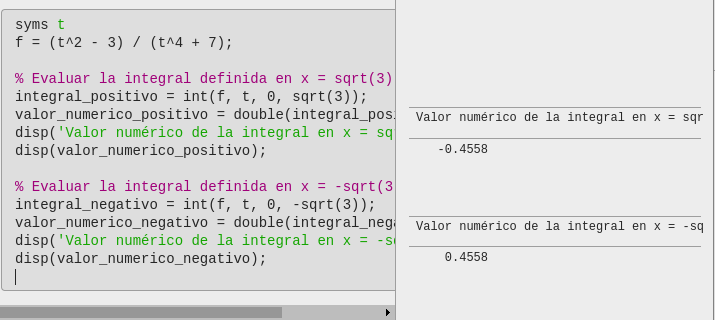
\includegraphics[height = 0.25\textheight]{recursos/ejercicio56.png}\par
\end{figure*}
$\therefore$ Concluimos que  $-\sqrt{3}$ es un máximo absoluto y $\sqrt{3}$ es un mínimo absoluto.

\newpage
d)Graficamos y Concluimos que es correcto
\begin{figure*}[!hbt]
	\centering
	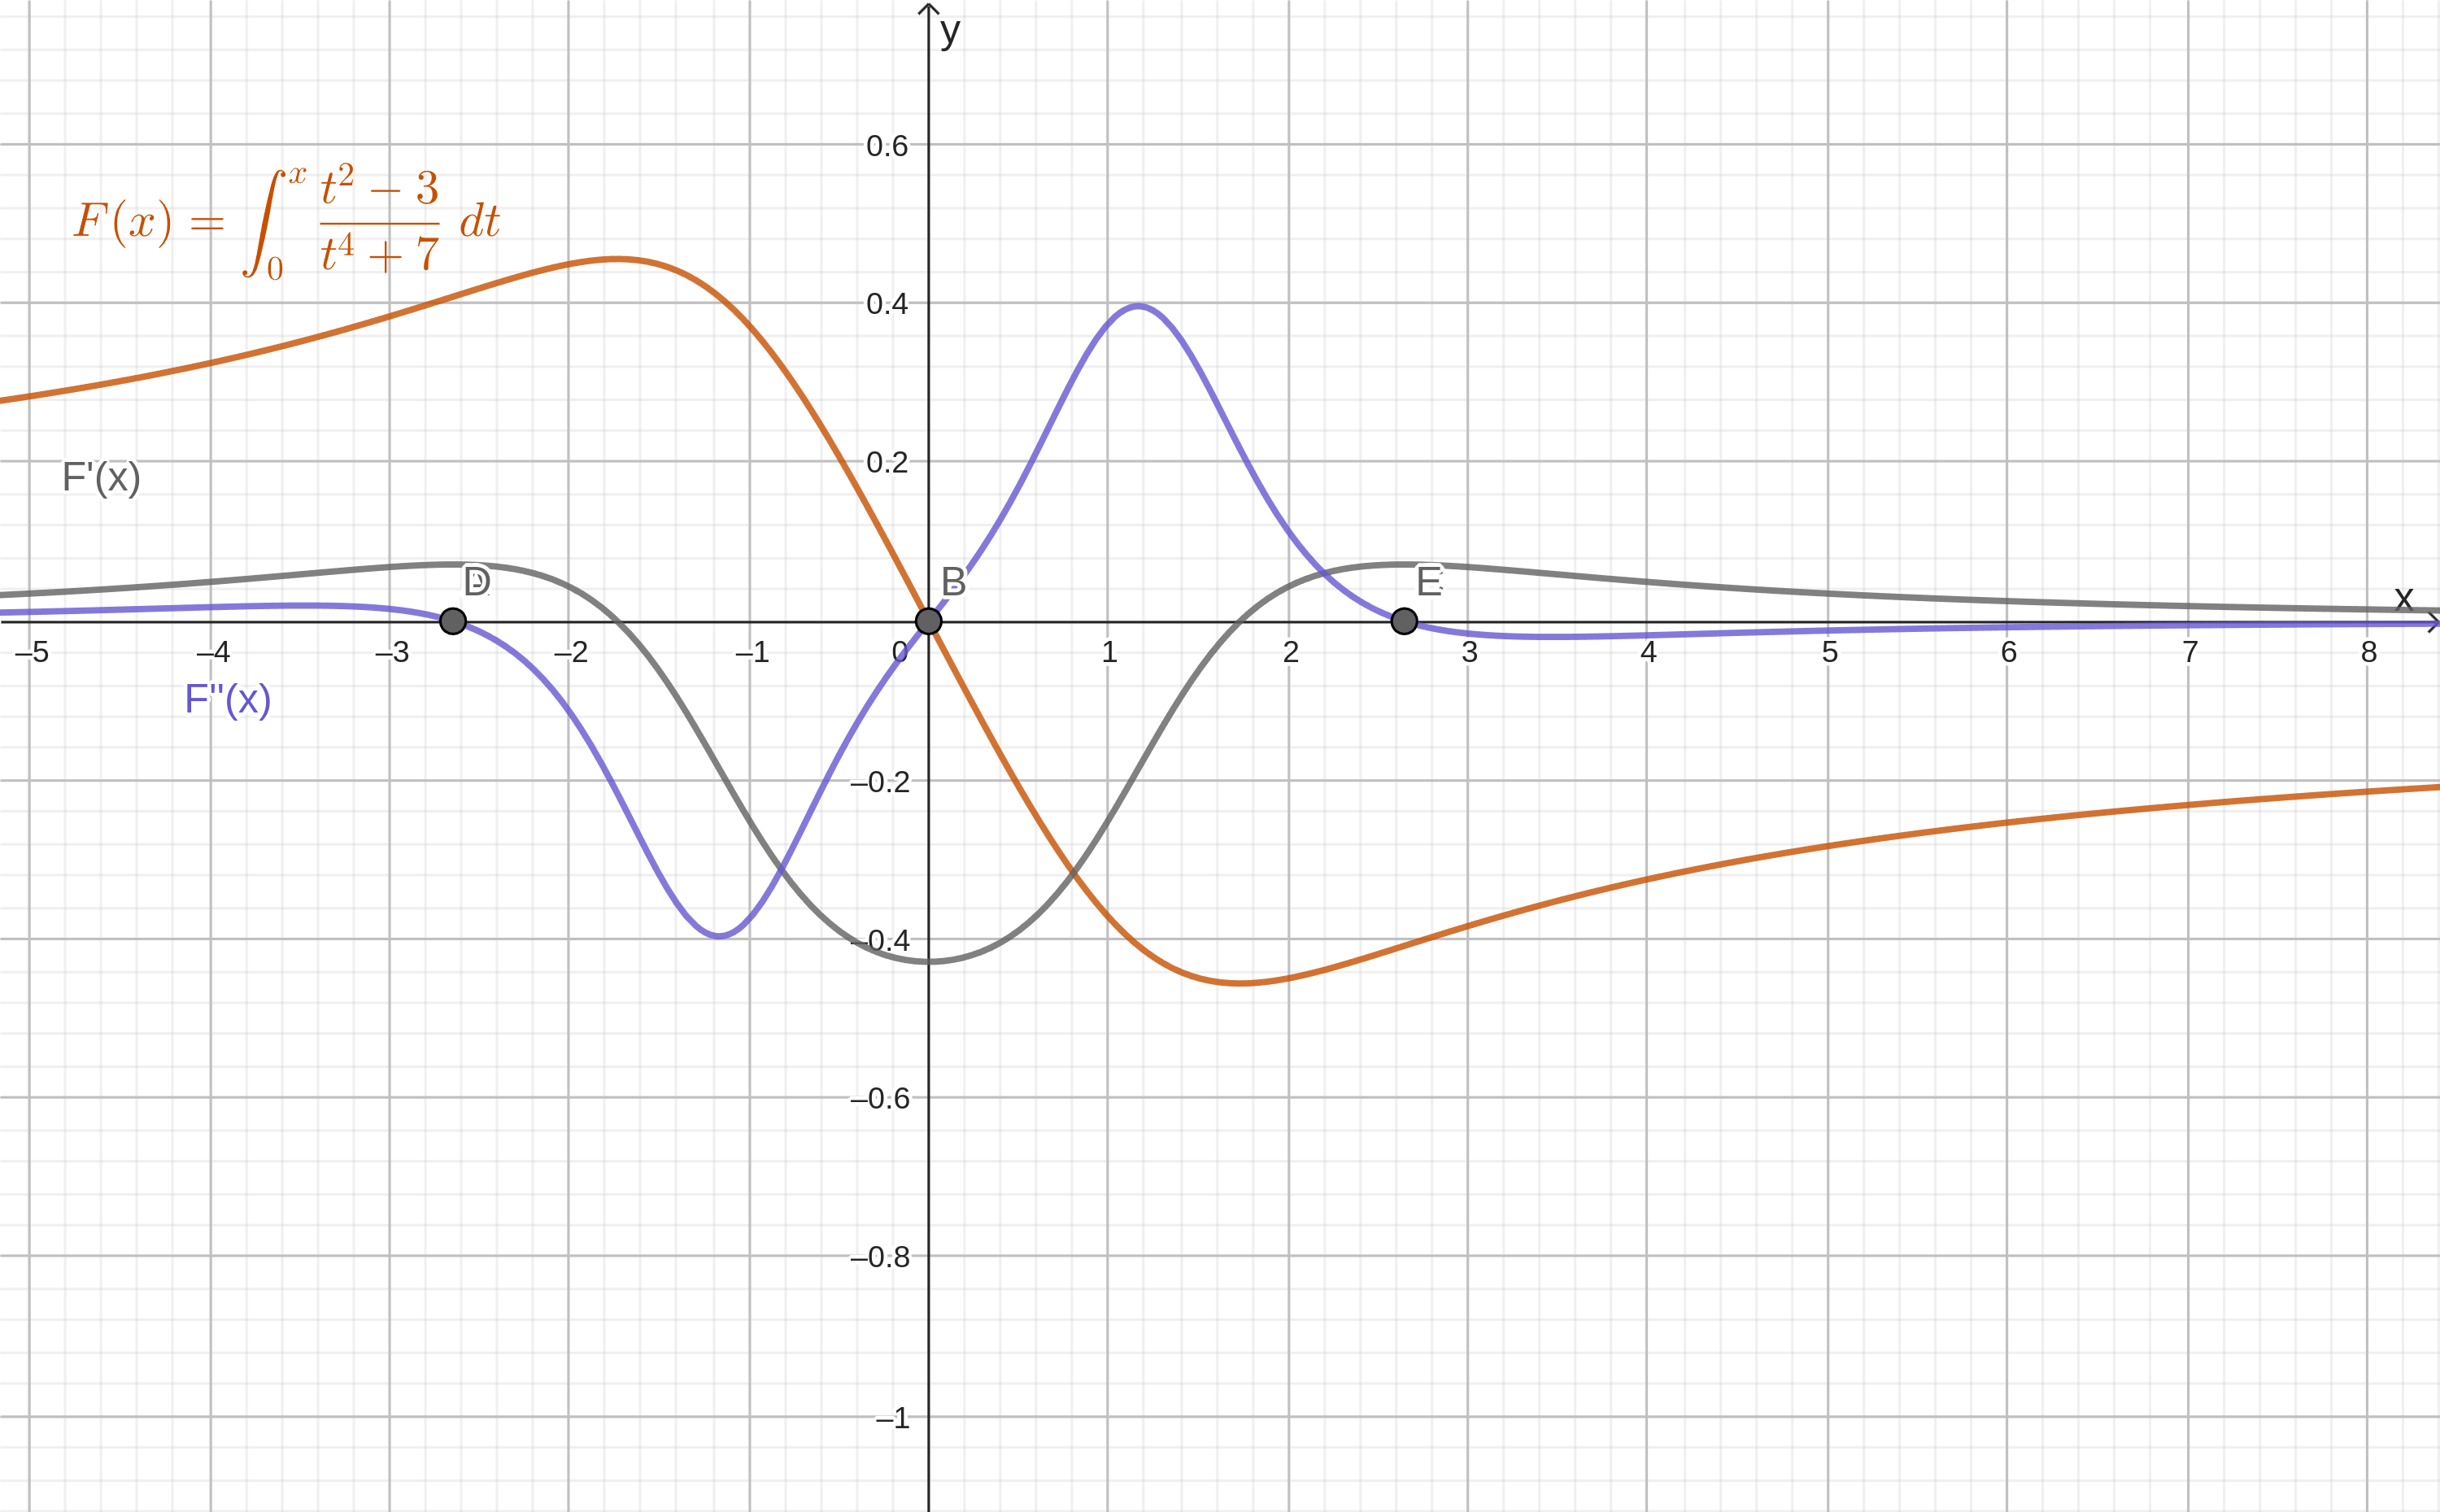
\includegraphics[height = 0.40\textheight]{recursos/ejercicio56_1.png}\par
\end{figure*}\newpage
\chapter*{73. Una partícula se mueve con una velocidad de $v(t)\frac{m}{s}$ a lo largo de un eje s. Halla el desplazamiento y la distancia recorrida por la partícula en el intervalo de un tiempo dado.}

Sabemos que la velocidad es la derivada de la posición.
Calcularemos la diferecia de las posiciones para tener el desplazamiento total.
Sea $v(t)=\displaystyle\frac{1}{2}-\frac{1}{t^2},1\leq t \leq 3 $
\begin{align*}
	x(3)-x(1)=\int_{1}^{3}v(t)dt & =\int_{1}^{3}\big(\frac{1}{2}-\frac{1}{t^2}\big)dt      \\
	                             & =\int_{1}^{3}\frac{1}{2}dt -\int_{1}^{3}\frac{1}{t^2}dt \\
	                             & =\frac{1}{2}t\bigg|_1^3-\int_{1}^{3}t^{-2}dt            \\
	                             & =\frac{1}{2}t\bigg|_1^3+t^{-1}\bigg|_{1}^{3}            \\
	                             & =\frac{1}{2}t\bigg|_1^3+\frac{1}{t}\bigg|_{1}^{3}       \\
	                             & =\frac{1}{2}t\bigg|_1^3+\frac{1}{t}\bigg|_{1}^{3}       \\
	                             & =\frac{3}{2}-\frac{1}{2}+\frac{1}{3}-1                  \\
	                             & =\frac{1}{3}\text{m. de desplazamiento}                 \\
\end{align*}
$\therefore$ el desplazamiento total es de  $\frac{1}{3}\text{m. de desplazamiento}$\\
Ahora sabemos que la posición se describe como $x(t)=\frac{t}{2}+\frac{1}{t}$

Podemos notar que el desplazamiento no siempre es en linea recta por lo que debemos preguntarnos: ¿Cuándo pasa que $v(t)=0$?
\begin{align*}
	v(t)=0\iff \frac{1}{2}-\frac{1}{t^2}=\iff \frac{1}{t^2} & =\frac{1}{2} \\
	\frac{2}{t^2}                                           & = 1          \\
	2                                                       & = t^2        \\
	t^2                                                     & = 2          \\
	t                                                       & =\sqrt{2}    \\
\end{align*}
Debemos evaluar t en los límites
\begin{align*}
	v(1)=\frac{1}{2}-1=-\frac{1}{2} \\
	v(3)=\frac{1}{2}-\frac{1}{3^2}=\frac{1}{2}-\frac{1}{9}=\frac{9-2}{18}=\frac{7}{18}
\end{align*}
Como la partícula fue cambiando de dirección después de que se detuviera, para hallar la distancia recorrida, debemos sumar las áreas por debajo y por encima del eje.
\begin{align*}
	distancia                                                                                                                        & =\bigg|x(3)-x(1)\bigg|=\int_{1}^{3}\big|\big(v(t)\big)\big|dt                                                                                                                                                      \\
	\therefore \int_{1}^{\sqrt{2}}\bigg|\frac{1}{2}-\frac{1}{t^2}\bigg|dt+\int_{\sqrt{2}}^{3}\bigg|\frac{1}{2}-\frac{1}{t^2}\bigg|dt & =\int_{1}^{\sqrt{2}}\frac{1}{t^2}-\frac{1}{2}dt+\int_{\sqrt{2}}^{3}\frac{1}{2}-\frac{1}{t^2}dt                                                                                                                     \\
	                                                                                                                                 & =\biggl[\int_{1}^{\sqrt{2}}t^{-2}dt-\int_{1}^{\sqrt{2}}\frac{1}{2}dt\biggr]+\biggl[\int_{\sqrt{2}}^{3}\frac{1}{2}dt-\int_{\sqrt{2}}^{3}t^{-2}dt\biggr]                                                             \\
	                                                                                                                                 & =\biggl[-\frac{1}{t}-\frac{t}{2}\biggr]\Bigg|_1^{\sqrt{2}}+\biggl[\frac{t}{2}-\frac{1}{t}\biggr]\Bigg|_{\sqrt{2}}^3                                                                                                \\
	                                                                                                                                 & =\biggl[\Biggl(-\frac{1}{\sqrt{2}}-\frac{\sqrt{2}}{2}\Biggr)-\Biggl(-\frac{1}{1}-\frac{1}{2}\Biggr)\biggr]+\biggl[\Biggl(\frac{3}{2}-\frac{1}{3}\Biggr)-\Biggl(\frac{\sqrt{2}}{2}-\frac{1}{\sqrt{2}}\Biggr)\biggr] \\
	                                                                                                                                 & =\biggl[-\frac{2\sqrt{2}}{2}+\frac{3}{2}\biggr]+\biggl[\frac{11}{6}-\frac{2\sqrt{2}}{2}\biggl]                                                                                                                     \\
	                                                                                                                                 & =-\sqrt{2}+\frac{3}{2}+\frac{11}{6}-\sqrt{2}                                                                                                                                    \\
	                                                                                                                                 & =\frac{3}{2}+\frac{11}{6}-2\sqrt{2}                                                                                                                                    \\
	                                                                                                                                 & =\frac{18+22}{12}-2\sqrt{2}\\
	                                                                                                                                 & =\frac{40}{12}-2\sqrt{2}\\
	                                                                                                                                 & =\frac{10}{3}-2\sqrt{2}\\
\end{align*}
Se concluye entonces que la distancia total recorrida por la praticula es $\displaystyle\frac{10}{3}-2\sqrt{2}\simeq 0.50490\;m$
\chapter*{capitulo 7 ejercicio 7}
\textbf{a) Estblesca una suma de integrales definidade que represente el área sombreada total entre las curvas $y=f(x)$ e $y=g(x)$ en la siguiente figura. b)Encuentra el área total encerrada entre $y=x^3$ e $y=x$ en el intervalo $[-1, 2]$.}
\begin{figure*}[!hbt]
	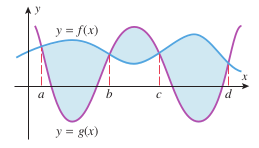
\includegraphics[height = 0.20\textheight]{recursos/image.png}\par
\end{figure*}

Si \( f \) y \( g \) son funciones continuas en el intervalo \([a, b]\), y si \( f(x) \geq g(x) \) para todo \( x \) en \([a, b]\), entonces el área de la región delimitada por \( y = f(x) \) arriba, \( y = g(x) \) abajo, a la izquierda por la línea \( x = a \), y a la derecha por la línea \( x = b \) es \[ A = \int_{a}^{b} [f(x) - g(x)] \, dx \]

Entonces se puede observar que $f(x)\geq g(x)$ en el intervalo $[a,b]$ $\therefore$ el área de la región dada  $f(x)$ y $ g(x)$ es $$A_1=\int_{a}^{b}\bigg[f(x)-g(x)\bigg]dx$$

Por otro lado se puede observar que $f(x)\leq g(x)$ $\forall x\in[b,c]$ $\therefore$ el área está dada como $$A_2=\int_{b}^{c}\bigg[g(x)-f(x)\bigg]dx$$

Del mismo modo, el análisis de la región acotada por el intervalo $[c,d]$, observamos que $f(x)\geq g(x)$ $\forall x\in[c,d]$ $\therefore$ el área se describe como $$A_3=\int_{c}^{d}\bigg[f(x)-g(x)\bigg]dx$$
Entonces el área total etá dada por la suma de estas tres áreas indiciduales tal que
$$A_T=\int_{a}^{b}\bigg[f(x)-g(x)\bigg]dx + \int_{b}^{c}\bigg[g(x)-f(x)\bigg]dx + \int_{c}^{d}\bigg[f(x)-g(x)\bigg]dx$$

De este modo tenemos en cuenta los casos cuando $f(x)\geq g(x)$ y $f(x)\leq g(x)$
\\
b)Encuentra el área total encerrada entre $y=x^3$ e $y=x$ en el intervalo $[-1, 2]$.
Sean $y=f(x)=x$ y $y=g(x)=x^3$
¿Cuándo pasa que son iguales?
\begin{align*}
	f(x)=g(x)\iff x_1 & =x_2^3       \\
	f(x)=g(x)\iff 0   & =x_2^3-x     \\
	f(x)=g(x)\iff 0   & =x(x-1)(x+1) \\
\end{align*}
Son iguales en $x=0$, $x=1$ y $x=-1$

\newpage Procedemos a hacee el análisis de desigualdedes
\begin{table}[!hbt]
	\begin{center}
		\begin{tabular}{| c | c | c | c | c |}
			\hline
			\multicolumn{5}{ |c| }{Análisis de los intervalos}                 \\ \hline
			intervalo   & Punto de prueba & $f(x)$      & $g(x)$ & desigualdad \\ \hline
			($-1,0]$    & -1/2            & $-1/2     $ & $-1/8$ & $f<g$       \\
			($0,1\big]$ & 1/2             & $     1/2$  & $1/8$  & $f>g$       \\
			($1,2\big]$ & 3/2             & $3/2    $   & $27/8$ & $f<g$       \\\hline
		\end{tabular}
		\caption{tabla de análsis de signos de las regiones }
		\label{tab: tabla de análsis de signos de las regiones }
	\end{center}
\end{table}

Entonces aplicando la definición anterior, el area total está dada por
\begin{align*}
	A_T & =\int_{-1}^{0}[g(x)-f(x)]dx+\int_{0}^{1}[f(x)-g(x)]dx+ \int_{1}^{2}[g(x)-f(x)]dx                                 \\
	A_T & =\int_{-1}^{0}[x^3-x)]dx+\int_{0}^{1}[x-x^3]dx+ \int_{1}^{2}[x^3-x]dx                                            \\
	A_T & =\int_{-1}^{0}x^3dx-\int_{-1}^{0}xdx+\int_{0}^{1}xdx-\int_{0}^{1}x^3dx+ \int_{1}^{2}x^3dx-\int_{1}^{2}xdx        \\
	A_T & =\bigg(\frac{x^4}{4}-\frac{x^2}{2}\bigg)\bigg|^0_{-1}+\bigg(\frac{x^2}{2}-\frac{x^4}{4}\bigg)\bigg|_0^1+ \bigg(\frac{x^4}{4}-\frac{x^2}{2}\bigg)\bigg|_1^2 \\
	A_T & =-\bigg(\frac{-1^4}{4}-\frac{-1^2}{2}\bigg)+\bigg(\frac{1^2}{2}-\frac{1^4}{4}\bigg)+ \bigg(\frac{2^4}{4}-\frac{2^2}{2}\bigg)-\bigg(\frac{1^4}{4}-\frac{1^2}{2}\bigg) \\
	A_T & =\frac{1}{4}+\frac{1}{4}+ \bigg(4-2\bigg)+\frac{1}{4} \\
	A_T & =\frac{1}{2}+ 2+\frac{1}{4} \\
	A_T & =0.5+ 2 +0.25\\
	A_T & =2.75\\
\end{align*}

el área total es 2.75 unidades de área
\chapter*{capitulo 6 ABD ejercicio 19}
Un resorte ejerce una fuerza de $0.5N$ cuando se estira $0.25m$ más allá de su lognitud natural. Suponiendo que e aplica la ley de Hooke.
a) ¿Cuánto trabajo se realizó para estirar el resorte hasta esta longitud?
b) ¿Cuánto más allá de su longitud natural se puede estirar el resorte con $25J$ de trabajo?

Sabemos que $W=\displaystyle\int_{a}^{b}F(x)dx$
donde $F=F(x)$ es la fuerza.
$\therefore$
\begin{align*}
	F=F(x)&=k\cdot x\\
	0.5&=k\cdot (0.25)\\
    \implies k&=\frac{0.5}{0.25}=2
\end{align*}
Susutituimos en la integral.
\begin{align*}
    W=\int_{0}^{0.25}2xdx&=2\int_{0}^{0.25}xdx\\
&= 2\frac{x^2}{2}\bigg|_{0}^{0.25}=x^2\bigg|_{0}^{0.25}\\
&=(0.25)^2=(\frac{1}{4})^2=\frac{1}{16}J
\end{align*}

Concluimos que $16J$ es el trabajo realizado.

b) ¿Cuándo pasa que $W=25J$?

Sabemos que el trabajo está descrito como la ecuación $W=x^2$ para nuetro resorte.\\
$\implies$ $x^2=25\iff x=\sqrt{25}=5\;m$ \\
Por lo tanto 5 m es la longitud a la que se estira el resorte al aplicarle un trabajo de $25 J$

\chapter*{capitulo 7 ejercicio 19}
\textbf{Evaluar la integral $\displaystyle\int_{0}^{1}\frac{x^3}{\sqrt{x^2+1}}dx$}\\
a) Usando integración por partes.\\
$\displaystyle\frac{x^3}{\sqrt{x^2+1}}=x^3(x^2+1)^{-\frac{1}{2}}$
$\therefore$ definimos las partes tales que
$u=x^2,\;dv=x(x^2+1)^{-\frac{1}{2}}dx,\;du = 2xdx $
\begin{align*}
	v             & =\int x(x^2+1)^{-\frac{1}{2}}dx                 \\
	              & u=x^2+1\; du=2xdx\implies xdx=\frac{1}{2}du     \\
	v             & =\frac{1}{2}\int u^{-1/2}du                     \\
	              & =\frac{1}{2}\frac{u^{1/2}}{\frac{1}{2}}=u^{1/2} \\
	\therefore v= & (x^2+1)^{1/2}
\end{align*}
$\therefore$ Aplicando la formula de integración por partes tenemos que
\begin{align*}
	x^2\cdot \sqrt{x^2 +1}\bigg|^1_0-                                & 2\int_{0}^{1}(x^2 +1)^{1/2}xdx                                 \\
	\text{definimos }u=x^2+1\; du=2xdx                               & \implies xdx=\frac{1}{2}du, u(0)=1\;u(1)=2                     \\
	\implies x^2\cdot \sqrt{x^2 +1}\bigg|^1_0-\int_{1}^{2}u^{1/2}du= & x^2\cdot \sqrt{x^2 +1}\bigg|^1_0-\frac{u^{3/2}}{3/2}\bigg|_1^2 \\
	=x^2\cdot \sqrt{x^2 +1}\bigg|^1_0-\frac{2}{3}u^{3/2}\bigg|_1^2=  & \sqrt{2}-\frac{2}{3}\bigg(2^{3/2}-1\bigg)                      \\
	=\sqrt{2}-\frac{4\sqrt{2}}+2{3}                                  & =\frac{3\sqrt{2}}{3}-\frac{4\sqrt{2}+2}{3}                     \\
	                                                                 & =\frac{3\sqrt{2}-4\sqrt{2}+2}{3}                               \\
	                                                                 & =\frac{-\sqrt{2}+2}{3}
\end{align*}

b)Usando la sustitución $\displaystyle u=\sqrt{x^2+1}$

$\implies u^2=x^2+1\therefore            x^2=u^2-1, 2xdx=2udu\implies  xdx=udu,   \;u(0)=1,\;u(2)=\sqrt{2}                                                                                    $
\begin{align*}
	\int_{0}^{1}\frac{x^3}{\sqrt{x^2+1}}dx & =\int_{0}^{1}\frac{x^2}{\sqrt{x^2+1}}xdx        & = & \quad \bigg(\frac{u^3}{3}-u\bigg)\bigg|_1^{\sqrt{2}}                              \\
	                                       & =\int_{1}^{\sqrt{2}}\frac{u^2-1}{u}udu          & = & \quad \bigg(\frac{\sqrt{2}^3}{3}-\sqrt{2}\bigg)-\bigg(\frac{1}{3}-1\bigg)         \\
	                                       & =\int_{1}^{\sqrt{2}}u^2-1du                     & = & \quad \bigg(\frac{2\sqrt{2}}{3}-\frac{3\sqrt{2}}{3}\bigg)+\bigg(\frac{2}{3}\bigg) \\
	                                       & =\int_{1}^{\sqrt{2}}u^2du-\int_{1}^{\sqrt{2}}du & = & \quad \frac{2\sqrt{2}-3\sqrt{2}+2}{3}                                             \\
	                                       & \quad  =\frac{-\sqrt{2}+2}{3}                                                                                                           \\
\end{align*}

\chapter*{capitulo 7 ejercicio 45}
\textbf{Aproxima la integral utilizando (a) la aproximación del punto medio $M_{10}$, (b) la aproximación trapezoidal $T_{10}$ y (c) la aproximación de la regla de Simpson $S_{20}$. En cada caso, encuentra el valor exacto de la integral y aproxima el error absoluto. Expresa tus respuestas con al menos cuatro decimales.}

Sea la integral $\displaystyle \int_{1}^{3}\frac{1}{\sqrt{x+1}}dx$\\
Calculemos la integral
\begin{align*}
	\int_{1}^{3}\frac{1}{\sqrt{x+1}}dx & =\int_{1}^{3}(x+1)^{-1/2}dx                             \\
	u=x+1, du=dx\implies,u(1)=2,u(3)=4 & \int_{2}^{4}u^{-1/2}du=\frac{u^{1/2}}{1/2}\bigg|_2^4    \\
	                                   & =2u^{1/2}\bigg|_2^4=2\sqrt{4}-2\sqrt{2}\simeq 1.1715728
\end{align*}
1) Aproximación con el punto medio ($M_{10}$)
\[\sum_{j=1}^{n}f(x^*_j)\Delta x=\Delta x\sum_{j=1}^{n}f(x^*_j)\]
donde $\Delta x = \frac{(b-a)}{n}$ y $x_j^*=a+(j-\frac{1}{2})\Delta x$\\
Definimos $\Delta x =\frac{3-1}{10}=\frac{1}{5}$ y $f(x)=\frac{1}{\sqrt{x+1}}$\\
$\displaystyle \int_{1}^{3}\frac{1}{\sqrt{x+1}}dx\approx \Delta x\sum_{j=1}^{n}f(x_j^*)=\Delta x\sum_{j=1}^{n}\frac{1}{\sqrt{(1+(j-\frac{1}{2})\Delta x)+1}}$

\begin{table}[!hbt]
	\begin{center}
		\begin{tabular}{| c | c | c | c | }
			\hline
			\multicolumn{4}{ |c| }{$n=10,\;\Delta x =\frac{1}{5}=0.2$}                                 \\ \hline
			i  & $(j-\frac{1}{2})\cdot \Delta x $ & $x_j=1+(j-\frac{1}{2})\cdot\Delta x$ & $f(x_{j})$  \\ \hline
			1  & 0.1                              & 1.1                                  & 0.690065559 \\
			2  & 0.3                              & 1.3                                  & 0.659380473 \\
			3  & 0.5                              & 1.5                                  & 0.632455532 \\
			4  & 0.7                              & 1.7                                  & 0.608580619 \\
			5  & 0.9                              & 1.9                                  & 0.58722022  \\
			6  & 1.1                              & 2.1                                  & 0.567961834 \\
			7  & 1.3                              & 2.3                                  & 0.550481883 \\
			8  & 1.5                              & 2.5                                  & 0.534522484 \\
			9  & 1.7                              & 2.7                                  & 0.519875245 \\
			10 & 1.9                              & 2.9                                  & 0.506369684 \\ \hline
			\multicolumn{4}{ |r| } {suma $ = 5.856913533\;$}                                           \\
			\multicolumn{4}{|r|}{$A\approx \Delta x \sum_{j=1}^{10}= 1.171382707$}                     \\ \hline
		\end{tabular}
		\caption{Metodo de Aproximación por el método del punto medio }
		\label{tab:Area por el método del punto medio}
	\end{center}
\end{table}
$\therefore$ el área con esta aproximación es $\displaystyle A\approx \Delta x \sum_{j=1}^{10}= 1.171382707$

$|EM | = | 4-2\sqrt{2} - M10 |= 1.171572875-1.171382707=0.000190169$
\\
2) Aproximación con el método trapezoidal ($T_{10}$)
\[\sum_{j=1}^{n}A(T_j)\Delta x=\frac{\Delta x}{2}\biggl[f(x_0)+2\sum_{j=1}^{n-1}f(x_{j})+f(x_n)\biggr]\]
donde $\Delta x = \frac{(b-a)}{n}=\frac{3-1}{10}=\frac{2}{10}=0.2$ y $x_j=a+j\Delta x$\\
Definimos $f(0)=f(a),f(x_j)=\frac{1}{\sqrt{x_j+1}}, f(n-1)=f(x_{n-1})=\frac{1}{\sqrt{x_{n-1}+1}}, f(n)=f(x_{n})=\frac{1}{\sqrt{x_{n}+1}}$\\
$\displaystyle \int_{1}^{3}\frac{1}{\sqrt{x+1}}dx\approx \frac{\Delta x}{2}\biggl[\frac{1}{\sqrt{a+1}}+2\sum_{j=1}^{n-1}\frac{1}{\sqrt{x_j+1}}+\frac{1}{\sqrt{x_n+1}}\biggr]$

\begin{table}[!hbt]
	\begin{center}
		\begin{tabular}{| c | c | c | c | }
			\hline
			\multicolumn{4}{ |c| }{$n=10,\;\Delta x =\frac{1}{5}=0.2$}                              \\ \hline
			i  & $x_j $ & $x_j=1+(j-\frac{1}{2})\cdot\Delta x$ & $f(x_{j})$                         \\ \hline
			0  & 1      & 0.707106781                          & 0.707106781                        \\
			1  & 1.2    & 0.674199862                          & 1.348399725                        \\
			2  & 1.4    & 0.645497224                          & 1.290994449                        \\
			3  & 1.6    & 0.620173673                          & 1.240347346                        \\
			4  & 1.8    & 0.597614305                          & 1.195228609                        \\
			5  & 2      & 0.577350269                          & 1.154700538                        \\
			6  & 2.2    & 0.559016994                          & 1.118033989                        \\
			7  & 2.4    & 0.542326145                          & 1.084652289                        \\
			8  & 2.6    & 0.527046277                          & 1.054092553                        \\
			9  & 2.8    & 0.512989176                          & 1.025978352                        \\
			10 & 3      & 0.5                                  & 0.5                                \\ \hline
			\multicolumn{4}{ |r| } {suma $ = 11.71953463\;$}                                        \\
			\multicolumn{4}{|r|}{$A\approx \frac{\Delta x}{2} \sum_{j=1}^{10}A(T_j)= 1.1719583463$} \\ \hline
		\end{tabular}
		\caption{Metodo de Aproximación por el método del trapecio }
		\label{tab:Area por el método del trapecio}
	\end{center}
\end{table}
$\therefore$ el área con esta aproximación es $\displaystyle A\approx \Delta x \sum_{j=1}^{10}= 1.1719583463$

$|EM | = | 4-2\sqrt{2} - T10 |= 1.171572875-1.1719583463=0.000380588$

3) Aproximación con la regla de Simpson($S_{10}$)\\
$\displaystyle\int_{a}^{b}v(t)dt\simeq \frac{b-a}{3n}\biggl[v(t_0)+4v(t_1)+2v(t_2)+\dotsc+2v(t_{2n-2})+4v(t_{2n-1})+v(t_{2n})\biggr]$

Se sugiere que si combinamos dos veces la aproximación del punto medio con la aproximación trapezoidal, los errores se cancelan entre sí.
Por lo tanto, la integral se puede aproximar como:
\[ S_n = \frac{1}{3} (2M_k + T_k),n=2k \]
Entonces, sustituyendo en la formula los resultados anteriormente dados
$$
S_{20}=\frac{1}{3} (2(1.171382707) + 1.1719583463) \\
	=\frac{1}{3}(3.514718876)\\
	=1.171572959$$
$|EM | = | 4-2\sqrt{2} - S20 |= 1.171572875-1.171572959=-8.35151*10^{-08}$

Como se puede observar, el error es casi nulo siendo un número muy pequeño.
\end{document}